% Exemplo de relatório técnico do IC
% Criado por P.J.de Rezende antes do Alvorecer da História.
% Modificado em 97-06-15 e 01-02-26 por J.Stolfi.
% Last edited on 2003-06-07 21:12:18 by stolfi
% modificado em 1o. de outubro de 2008
% modificado em 2012-09-25 para ajustar o pacote UTF8. Contribuicao de
%   Rogerio Cardoso

\documentclass[11pt,twoside]{article}
\usepackage{techrep-ic}
\usepackage{graphicx}
\usepackage{wrapfig}

%%% SE USAR INGLÊS, TROQUE AS ATIVAÇÕES DOS DOIS COMANDOS A SEGUIR:
\usepackage[brazil]{babel}
%% \usepackage[english]{babel}

%%% SE USAR CODIFICAÇÃO LATIN1, TROQUE AS ATIVAÇÕES DOS DOIS COMANDOS A
%%% SEGUIR:
%% \usepackage[latin1]{inputenc}
\usepackage[utf8]{inputenc}

\begin{document}

%%% PÁGINA DE CAPA %%%%%%%%%%%%%%%%%%%%%%%%%%%%%%%%%%%%%%%%%%%%%%%
% 
% Número do relatório
\TRNumber{00}

% DATA DE PUBLICAÇÃO (PARA A CAPA)
%
\TRYear{16}  % Dois dígitos apenas
\TRMonth{11} % Numérico, 01-12

% LISTA DE AUTORES PARA CAPA (sem afiliações).
\TRAuthor{H. Freitas \and V. Oliveira}

% TÍTULO PARA A CAPA (use \\ para forçar quebras de linha).
\TRTitle{Gerenciamento de Redes Autonômicas e Cognitivas}

\TRMakeCover

%%%%%%%%%%%%%%%%%%%%%%%%%%%%%%%%%%%%%%%%%%%%%%%%%%%%%%%%%%%%%%%%%%%%%%
% O que segue é apenas uma sugestão - sinta-se à vontade para
% usar seu formato predileto, desde que as margens tenham pelo
% menos 25mm nos quatro lados, e o tamanho do fonte seja pelo menos
% 11pt. Certifique-se também de que o título e lista de autores
% estão reproduzidos na íntegra na página 1, a primeira depois da
% página de capa.
%%%%%%%%%%%%%%%%%%%%%%%%%%%%%%%%%%%%%%%%%%%%%%%%%%%%%%%%%%%%%%%%%%%%%%

%%%%%%%%%%%%%%%%%%%%%%%%%%%%%%%%%%%%%%%%%%%%%%%%%%%%%%%%%%%%%%%%%%%%%%
% Nomes de autores ABREVIADOS e titulo ABREVIADO,
% para cabeçalhos em cada página.
%
\markboth{Freitas, Humberto e Oliveira, Vitor}{Redes Autonômicas}
\pagestyle{myheadings}

%%%%%%%%%%%%%%%%%%%%%%%%%%%%%%%%%%%%%%%%%%%%%%%%%%%%%%%%%%%%%%%%%%%%%%
% TÍTULO e NOMES DOS AUTORES, completos, para a página 1.
% Use "\\" para quebrar linhas, "\and" para separar autores.
%
\title{Gerenciamento de Redes Autonômicas e Cognitivas}

\author{Humberto Silva Galiza de Freitas\thanks{Rede Nacional de Ensino e Pesquisa (RNP), 
Av. Dr Andre Tosello, 209, 13083-886, Campinas, SP.} \and
Vitor Correa Oliveira\thanks{Instituto  de Computação, Universidade
Estadual  de Campinas, 13081-970, Campinas, SP. }}

\date{}

\maketitle

%%%%%%%%%%%%%%%%%%%%%%%%%%%%%%%%%%%%%%%%%%%%%%%%%%%%%%%%%%%%%%%%%%%%%%

\begin{abstract} 
  Este trabalho é um relatório técnico de um projeto temático 
  desenvolvido na disciplina MOB655, visando fornecer uma visão geral
  das Redes Autonômicas bla bla blabla bla blabla bla blabla bla blabla bla blabla bla bla
  bla bla blabla bla blabla bla blabla bla blabla bla blabla bla blabla bla blabla bla blabla bla bla
  bla bla blabla bla blabla bla blabla bla blabla bla blabla bla blabla bla blabla bla blabla bla blabla bla blav
  bla bla blabla bla blabla bla blabla bla blabla bla blabla bla blabla bla blabla bla blabla bla bla
  bla bla blabla bla blabla bla blabla bla blabla bla blabla bla blabla bla blabla bla bla.
\end{abstract}

\section{Introdução}
A inspiração da computação autonômica vem do sistema nervoso autônomo dos animais, elemento responsável pela maioria das funções vitais de controle de um organismo vivo. Esse sistema atua na coordenação e regulação das atividades corporais de uma maneira inteligente e inconsciente. 

Exemplos da atuação desse sistema são os movimentos involuntários dos tecidos do coração, dos músculos do sistema respiratório, e bem como as reações automáticas desencadeadas pelo corpo humano em resposta a alterações ambientais, tais como a presença de luz e variações de temperatura, de modo a manter o seu equilibrio. A Figura~\ref{Sec:Intro:Fig1} mostra alguns exemplos de ações desempenhadas pelo sistema nervoso autônomo no corpo humano.

\begin{figure}
    \centering
    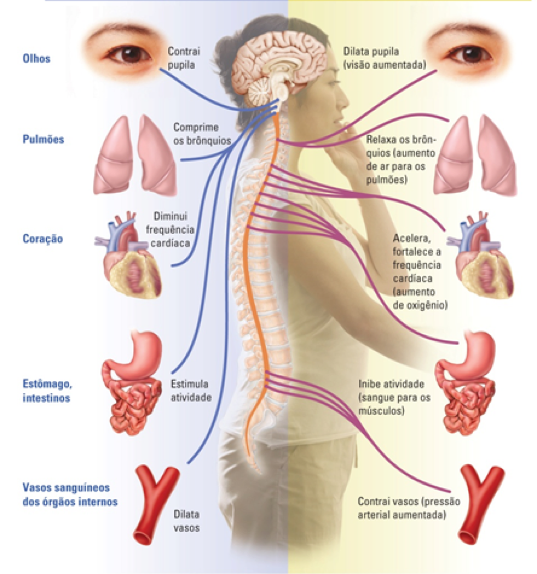
\includegraphics[width=0.5\textwidth]{Picture1.png}
    \caption{Sistema nervoso autônomo humano.}
    \label{Sec:Intro:Fig1}
\end{figure}

O conceito de computação autonômica foi apresentado inicialmente pela IBM em 2001~\cite{KEPHART}, e indicava que o crescimento na complexidade e heterogeneidade de gerenciamento dos ambientes computacionais consistia no principal problema a ser atacado pela computação autonômica. 

Assim, a computação autonômica pode ser descrita como um sistema capaz de se auto-organizar conforme as regras de negócio e objetivos definidos pelos administradores~\cite{ROMILDO}. Para alcançar esse nível de auto-gerenciamento, quatro áreas básicas devem ser atendidas: auto-configuração (\textit{Self-Configuration}), auto-otimização (\textit{Self-Optimization}), auto-cura (\textit{Self-Healing}) e auto-proteção (\textit{Self-Protection}).

\subsection{Princípios e Terminologia}
Os principios que norteiam os sistemas autonômicos foram inicialmente descritos no trabalho de \textit{Paul Horn}~\cite{KEPHART}, cientista e vice-presidente de pesquisa da IBM, em março de 2001, na Academia Nacional de Engenheiros de Havard. 

Segundo o autor, quatro peças fundamentais compõe os requisitos para o auto-gerenciamento de um sistema autonômico, a saber:

\begin{itemize}

\item Auto-Configuração (\textit{Self-Configuration}) - Os sistemas autonômicos devem possuir a capacidade de configurar e reconfigurar-se de acordo com variações externas, previstas ou não. A auto-configuração não deve se limitar à capacidade de um sistema configurar cada dispositivo isoladamente, mas deve ser capaz de prover o ajuste de configuração dos dispositivos dinamicamente.

\item Auto-Otimização (\textit{Self-Otimization}) - Os sistemas autonômicos devem sempre estar em busca de otimização de seu trabalho, identificando novas oportunidades de aperfeiçoamento do seu trabalho, com melhor desempenho ou menor custo utilizando os mesmos recursos disponíveis.

\item Auto-Cura (\textit{Self-Healing}) - Os sistemas autonômicos devem possuir capacidade de recuperar-se quanto atingidos por eventos que venham prejudicar o seu bom funcionamento, assim como detectar e aplicar soluções para que os problemas sejam corrigidos. 

\item Auto-Proteção (\textit{Self-Protection}) - Os sistemas autonômicos devem possuir um bom conhecimento sobre o ambiente que está a sua volta, a fim de inteirar-se com sistemas próximos, de forma a se antecipar a problemas baseando-se na correção de dados e/ou estudo dos seus estudos anteriores. A Auto-Proteção também pode estar associada à capacidade de reconhecer e lidar com condições de sobrecarga que possam comprometer a integridade do sistema.
\end{itemize}

Além disso, os sistemas autonômicos devem possuir um bom conhecimento sobre o ambiente que está a sua volta a fim de inteirar-se com sistemas vizinhos e com o ambiente que o cerca. Essa propriedade é denominada Auto-Consciência (\textit{Self-Awareness}).

Espera-se de um sistema autonômico a possibilidade de propor novas soluções de acordo com o estado atual do ambiente gerenciado, mesmo que não existam pré-configurações para tal estado. Por isso, na literatura, há uma diferenciação entre sistema automático e sistema autonômico. 

Em linhas gerais, um sistema automático é capaz de reagir a mudanças de contexto de um conjunto de estados pré-definidos, e geralmente esse tipo de sistema está vinculado ao conceito de automação. Por outro lado, um sistema autonômico deve se autoconfigurar mesmo em situações não previsíveis, de forma a tentar manter o desempenho, mesmo com falhas, não se contentando com o \textit{status quo}~\cite{GANEK}.


\section{Gerenciamento de Redes Autonômicas}
Quando se fala em sistemas autonômicos podemos fazer um paralelo com o corpo humano, pois, este possui diversos sistemas (Ex: respiratório, digestivo dentre outros) compostos por órgãos do qual estão interconectados, já os sistemas autonômicos possuem diversos componentes, físicos ou lógicos, com importantes funções e com a finalidade de exercerem bem seu papel para que o todo funcione de forma perfeita.

Os sistemas, em sentido amplo, com o passar do tempo tendem a evoluir fazendo com que fique cada vez mais complexo seu processo de gerenciamento além de dificultar manutenção da qualidade dos serviços oferecidos. Eis que surge a ideia de sistemas com capacidade de auto-gerenciamento, diminuindo a função ativa do administrador (ser humano) e passando o para uma função de supervisão.

\subsection{Estudo comparativo}
%Revisar essa subseção
%Traçando-se um paralelo entre a computação atual e a computação autonômica, temos que
%a.	Comparativo
%Computação Atual:
%1.	Centro de dados corporativos com múltiplos fornecedores. [Auto-Configuração]
%2.	Instalação, configuração e integração de sistemas podem ser demorada e propensa a erros. [Auto-Configuração]
%3.	Parâmetros de sistemas são definidos manualmente além de aumentar consideravelmente a cada nova versão. [Auto-Otimização]
%4.	Detecção de problemas em sistemas complexos pode demorar por semanas para serem encontrados pela equipe de programadores. [Auto-Cura]
%5.	Detecção e recuperação de ataques é feita manualmente. [Auto-Proteção]
%Computação Autonômica:
%1.	Configuração automatizada de componentes e sistemas seguindo uma política de alto nível. [Auto-Configuração]
%2.	Componentes e sistemas buscam continuamente a melhora de desempenho e eficiência. [Auto-Otimização]
%3.	O sistema faz a detecção, diagnostico e reparo de problemas em software e hardware [Auto-Cura]
%4.	Sistema faz automaticamente a defesa contra ataques maliciosos e falhas em cascata. [Auto-Proteção]
%5.	Sistema faz uso de alertas de previas para antecipar falhas em todo o sistema. [Auto-Proteção]

%a.	Diferenças:
%a.	Autonômicos: Caracterizam-se por gerenciar a si próprio além de possuírem capacidade de aprendizado através de sua experiência, este último fator é um ponto que separa os sistemas autônomos dos autonômicos.

%b.	Automáticos: Caracterizam-se por respostas ou soluções pré-definidas, por exemplo: Caso ocorra algum tipo de problema este tipo de sistema poderá solucionar o ocorrido, desde que a solução esteja pré-definida sendo essa uma característica vital, pois em sistemas automáticos não existe a capacidade de autoaprendizagem.
FALTA FAZER UM TEXTO EXPLICANDO AS DIFERENCAS

\subsection{Níveis de Automaticidade}
Os sistemas autonômicos evoluem de forma gradativa, e as evoluções deste paradigma devem ser feitas de maneira progressiva, ou seja, são necessárias atualizações de softwares, ferramentas e processos sendo que isso leva um certo tempo e deve ser feito de forma planejada e cuidadosa. 
\begin{figure}
    \centering
    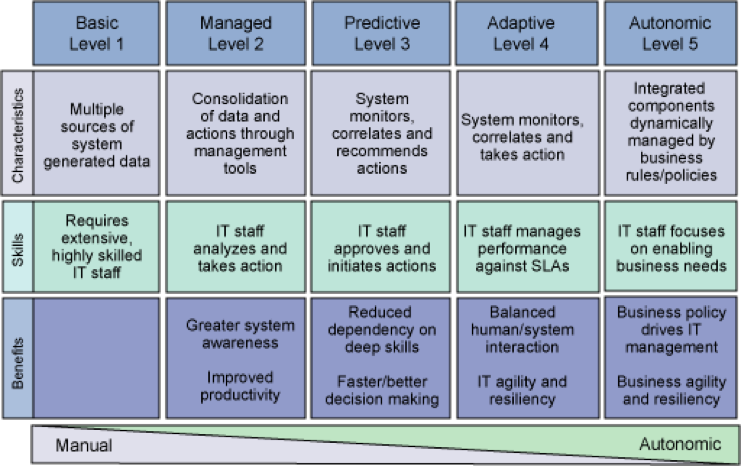
\includegraphics[width=0.6\textwidth]{Picture2.png}
	\caption{Níveis de automaticidade}
    \label{Sec:Intro:Fig2}
\end{figure}
Durante este período de maturação devem ser resolvidos alguns desafios com relação ao paradigma autonômico como por exemplo as variáveis de diferentes origens que um sistema pode ter que equacionar para resolver um determinado problema. 

\subsubsection{Básico}
A gerência é caracterizada por processos manuais, em que os administradores do sistema devem ser os responsáveis pela configuração, monitoramento e correção nos casos de falhas. 

Pontos negativos: 
\begin{itemize}
\item Neste nível vários profissionais são necessários manterem os sistemas.
\item O processo é manual e reativo.
\end{itemize}

A eficiência neste nível é mensurada pelo tempo utilizado pelo administrador nas soluções dos problemas.

\subsubsection{Gerenciado}
O nível gerenciado é caracterizado pela presença de tecnologias de gerenciamento de sistemas, com isso a coleta de informações é feita através do próprio sistema e são utilizadas para planejamento e tomada de decisões futuras dos administradores de sistemas. Neste nível as informações são documentadas e são melhoradas no decorrer do tempo.
Ponto negativo:
\begin{itemize}
\item O processo ainda é manual.
\end{itemize}

A eficiência neste nível é mensurada através do tempo em que o sistema está disponível e tempo necessário para encerrar possíveis problemas ou requisições.

\subsubsection{Preditivo}
Neste terceiro nível de gerenciamento, é marcado pela comunicação entre diversos elementos de um sistema através de tecnologias e protocolos que abarquem a maior quantidade possível de dispositivos. Os administradores são melhores auxiliados neste modelo, pois o processo é pró-ativo, ou seja, existe um ciclo de aprovação menor além de que as ferramentas existentes analisam e sugerem recomendações para os dispositivos.

A eficiência neste nível será mensurada através da disponibilidade dos sistemas, de SLAs (Service Level Agreements) e avaliação dos clientes do serviço.

\subsubsection{Adaptativo}
No nível adaptativo pode-se dizer que há uma interligação com o nível anterior, preditivo, e também podemos considerar que esta é a última etapa antes de um gerenciamento totalmente autonômico verdadeiramente, uma vez que os sistemas podem realizar ações automaticamente baseando-se no conhecimento obtido do que está acontecendo e do ambiente que o cerca. 

As ações executadas neste nível devem seguir as SLAs (Service Level Agreements), uma vez que são utilizadas ferramentas de gerenciamento que são baseadas em políticas.
A avaliação de eficiência neste nível será similar com a do nível anterior, preditivo, ou seja, satisfação de clientes, atendimentos de SLAs e tempo de resposta com relação aos sistemas, mas com um fator diferencial que será a contribuição do serviços de TI para o sucesso de negócio.

\subsubsection{Autonômico}
Este é o nível mais elevado que um sistema pode chegar, uma vez que existe por completo o auto-gerenciamento. O sistema é gerenciado por políticas e objetivos de negócio, aqui o administrador do sistema possui a atribuição de monitoramento do processo como um todo e quando julgar necessário pode alterar os objetivos. 

Neste último nível são aplicadas todas as melhores praticas para o gerenciamento de TI além destas serem automatizadas, é levado em conta também pelas ferramentas de análise os custos e a análise de compromissos.

A eficiência no nível mais elevado de autonomicidade é feito de acordo com o sucesso do negócio, das métricas de SLAs e das taxas de retorno do negócio.

\subsection{Elemento Autonômico}
É a menor parte de um sistema autonômico, este pode estar presente em diversos dispositivos que proveem serviços para outros elementos autonômicos ou seres humanos. Uma das características de um elemento autonômico é o fato deste possuir um único gerente responsável pelo monitoramento dos elementos gerenciados. 

\begin{figure}
    \centering
    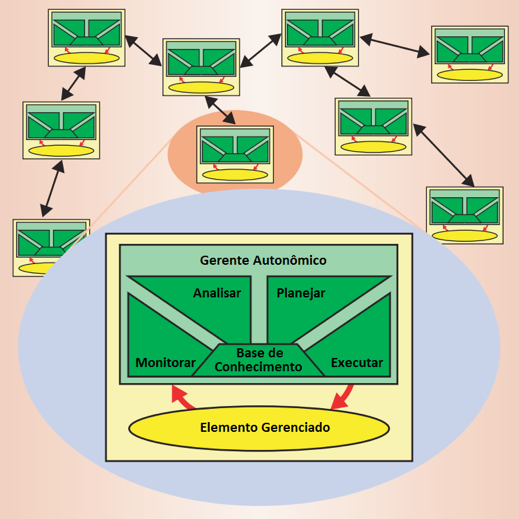
\includegraphics[width=0.5\textwidth]{Picture3.png}
    \caption{Gerenciamento do elemento autonômico~\cite{KEPHART}.}
    \label{Sec:Intro:Fig3}
\end{figure}

Em uma rede autonômica existem diversos componentes que possuem a capacidade de se controlar e monitorar, neste cenário cada elemento autonômico deverá atuar para promover da melhor forma possível os recursos do componente na rede da qual está inserido e tudo isso sem diminuição da qualidade de serviço.

\subsection{Gerenciamento do Elemento Autonômico}
Há um modelo genérico proposto por~\cite{KEPHART} demonstrando a na Figura~\ref{Sec:Intro:Fig3}, no qual diz que um elemento autonômico deverá conter uma base de conhecimento para armazenar as seguintes informações: dados, parâmetros e limitadores. Neste modelo o gerente do elemento autonômico descrito anteriormente deverá percorrer continuamente as informações referentes ao monitoramento e a análise dos dados internos e externos dos elementos gerenciados.

Conforme demonstrado na Figura~\ref{Sec:Intro:Fig3}, o gerenciador autonômico possui cinco partes que são: Monitoração, Análise, Planejamento, Execução e Base de Conhecimento. A seguir, cada uma dessas partes serão detalhadas.

\subsubsection{Monitoração} 
Quando se fala em gerenciamento é fundamental o processo de monitoramento, pois não é possível gerenciar algo que não se tenha conhecimento. Nesta etapa são aplicados os serviços de autoconhecimento e autoconsciência, este indica que o componente gerenciado deve conhecer os que estão ao seu redor, ou seja, sua vizinhança, já aquele deverá conhecer a si próprio e seus componentes. 

Um bom exemplo de monitoramento em ambientes tradicionais são os de hardware, por exemplo CPU, ou de software, por exemplo, Banco de Dados. As informações obtidas deste monitoramento devem ser enviadas para uma base de conhecimento.

\subsubsection{Análise}
Está fase é responsável por transformar os dados obtidos na fase de monitoramento em informações desejadas, estando armazenadas na base de conhecimento conforme mencionado anteriormente. Espera-se que estas informações possibilitem a conclusões sobre diversos aspectos, dentre eles detecção de possíveis problemas ou até mesmo a previsão de modificações futuras no sistema.

\subsubsection{Planejamento}
O principal objetivo desta fase é traçar estratégias de mudanças caso necessário de acordo com o resultado obtido da analise realizada pelo serviço anterior. Nesta fase podemos também mencionar diversos serviços de gerenciamento que terão funções importantes como, por exemplo: Auto sustento, auto-manutenção, auto-organização dentre outros, e com o auxilio destes serviços é nesta fase que será definido o planejamento e a ordem de execução das ações a serem tomadas.

\subsubsection{Execução}
Esta fase deverá executar as tarefas de configuração ou reconfiguração da melhor forma possível em elementos como, por exemplo: hardware ou software, isto é feito de acordo com um dos principais aspectos do tópico computação autonômica: a auto-configuração. Não é de responsabilidade desta fase fazer o planeamento referente a execução, aqui basta ser executado o plano da forma em que recebido pela etapa anterior e quando necessário fazer o tratamento de possíveis falhas durante a realização da tarefa. Caso haja falha durante a execução de alguma tarefa, está fase deverá executar ações de forma ordenada a fim de que uma destas apresente resultado satisfatório.

\subsubsection{Base de Conhecimento}
Está é uma das fases mais importantes do modelo genérico proposto por [Kaphart 2003], pois a base de conhecimento será responsável pelo armazenamento de dados, informações, políticas dentre outros elementos.

A base de conhecimento deverá conter quatro componentes: 
\begin{enumerate}

\item	Base de informações para gerenciamento local (\textit{Management Information Base} - MIB).
Finalidade: É utilizado para o armazenar dados de um elemento gerenciados de rede.

\item.	Base de Informações da Aplicação (AIB – Application Information Base).
Finalidade: Armazenar informações resultantes de uma aplicação ou aplicações executadas em um contexto autonômico (exemplo: uma rede).

\item Máquina de políticas. 
Finalidade: Está máquina deverá ser capaz de incluir, armazenar, atualizar, executar, excluir e selecionar políticas de acordo com a necessidade.

\item Módulo correspondente de gerenciamento utilizado. (\textit{Communication Protocol Base} - CPB)
\end{enumerate}

O ciclo de vida de elemento autonômico é dividido em 4 fases e cada uma destas serão descritas a seguir, das quais possuem problemas e desafios a serem superados. Um elemento autonômico possui seu ciclo de vida iniciado com a sua concepção e implementação, superada esta etapa inicial vai para parte de testes e verificação, prossegue para instalação, configuração, otimização, atualização, monitoramento, determinação de problemas e recuperação e finaliza seu ciclo com a desinstalação ou substituição do mesmo.

\subsubsection{Design, Teste e Verificação}
A fase de design em um projeto de elemento autonômico consiste na representação das necessidades de utilização de serviços de outros componentes, funcionalidades e capacidades, ou seja, o objetivo é propiciar aos projetistas ferramentas que os auxiliem para o mapeamento de ações de níveis inferiores. Já a fase de teste e verificação visa avaliar as funções executadas pelos elementos autonômicos. Esta fase é de suma importância uma vez que aqui é possível observar o comportamento de um elemento autonômico.

\subsubsection{Instalação e Configuração}
O Elemento Autonômico deverá incluir em um diretório de serviço um registro com detalhes referentes ao sua capacidade e informações de contatos, com isso os demais elementos da rede podem fazer uso deste diretório a fim de descobrir fornecedores e consumidores de informações e serviços.

\subsubsection{Monitoração e Determinação de Problemas}
Esta é uma fase fundamental no ciclo de vida de um elemento autonômico, pois segundo~\cite{KEPHART}, é neste momento que se torna possível através do laço de controle executado continuamente em espaços de tempo regulares, verificar e certificar-se que os objetivos estão sendo cumpridos. 

Ainda segundo~\cite{KEPHART} é possível trabalhar de forma pró-ativa, uma vez que o elemento pode fazer o monitoramento de outros componentes com a finalidade de evitar falhar além de conhecer a melhor condição do sistema como um todo. Nesta fase ainda pode ocorrer situações e que seja necessário determinar o motivo da falha, e para isso podem ser utilizadas as ferramentas de simulação e determinação de problemas em ambientes complexos, já que se deve evitar desligar e ligar novamente os componentes.
\subsubsection{Atualização}
As atualizações dos Elementos Autonômicos devem ser perene, ou seja, é necessária a atualização regular e contínua, sendo que isso é um desafio não trivial, pois quando há a identificação de que o Elemento Autonômico está desatualizado este precisa buscar novas atualizações disponíveis e incorporá-las em si próprio.

\subsubsection{Desinstalação e Reposição}
Todas as tarefas já mensionadas anteriormente referentes ao ciclo de vida são realizadas de forma contínua. Completado o ciclo de instalações e atualizaçÕes o Elemento Autonômico deverá identificar a necessidade de sair da rede e consequentemente ser desinstalado e substituído alem de retirar do diretório de serviço, este mensionado na parte de "Instalação e Configuração", seus recursos e serviços ofertados e finalizar todos os acordos de serviços firmados com os demais Elementos da rede.

\subsection{Desafios no Gerenciamento de Redes Autonômicas}
INCLUIR RESUMO DOS DESAFIOS - TESE DO ROMILDO

%\section{Gerência de Redes Autonômicas}
%a.	Auto-Configuração:
%Para o bom funcionamento de um elemento de seu sistema, este em sentido amplo, é vital que sua configuração esteja correta. A instalação, a integração e as configurações devem ser feitas de forma eficiente, sendo estas seguidas de políticas pré-estabelecidas.
%b.	Auto-Otimização:
%Ajustes de parâmetros a fim de que os sistemas operem da melhor maneira possível, é valido ressaltar que uma parametrização equivocada com a finalidade de otimizar um sistema ou rede poderá causar resultados catastróficos em todos os sistemas, uma vez que estes estão inter-conectados.
%c.	Auto-Cura:
%Redes ou sistemas podem apresentar falhas que podem causar prejuízos incalculáveis, sendo necessário o investimento em pesquisas para criação de soluções capazes de identificar e corrigir estas falhas de forma automatizada causando o mínimo de impacto para os usuários e empresas.
%d.	Auto-Proteção:
%As redes autonômicas devem ser especialistas em auto-proteção, sendo assim elas deverão fazer a sua defesa de duas formas: 
%•	Defesa contra ataques maliciosos: Ou seja, deverá defender o sistema como um todo a fim de evitar problemas de larga escala.
%•	Falhas em cascatas: Permanência de erros causados por medidas de auto-cura.
%É válido ressaltar também que as redes devem trabalhar de forma pró-ativa a fim de evitar problemas baseando se em informações anteriores e tomando medidas para evitar ou minimizar os impactos.
%e.	Auto-Conhecimento:
%Uma rede autonômica além de conhecer a si própria deverá também conhecer os componentes que a compõe, ou seja, esta deverá saber sobre configuração, parâmetros, serviços providos dentre outros itens que devem ser amplamente conhecidos pelo gerente autonômico responsável pelos recursos gerenciados. 
%f.	Auto-Consciência:
%Conforme apresentado no item anterior, além do conhecimento dos próprios recursos da rede, é necessário ter pleno conhecimento sobre o ambiente que o cerca, ou seja, a vizinhança da rede. Este tópico e de suma importância para as redes autonômicas, pois as ações tomadas pelo gerente autonômico são de acordo com o conhecimento interno (auto-configuração) quanto à configuração do ambiente externo, sua vizinhança.
%g.	Auto-Aprendizado:
%	(falta fazer.)
%h.	Auto-Diagnóstico:
%(falta fazer.)
%i.	Auto-Recuperação:
%	(falta fazer.)
%j.	Auto-Organização:
%(falta fazer.)
%k.	Auto-Serviço:
%l.		(falta fazer.)
%m.	Auto-Sustento:
%	(falta fazer.)
%n.	Auto-Manutenção:
%	(falta fazer.)

\section{Casos de uso}
Os conceitos de redes autonômicas podem ser aplicados em diversos modelos de redes, exemplo:
\begin{itemize}
	\item Redes WAN, LAN, MAN, PAN;
	\item Redes de telecomunicações.
	\item Redes móveis.
	\item Redes com ou sem fio.
\end{itemize}
Mas é valido ressaltar que cada modelo de rede possui as suas particularidades dentre elas protocolos específicos, objetivos diferentes, serviços e tecnologias distintas. Um bom exemplo disso é uma rede sem fio de um provedor de internet do qual necessita atender uma gama de clientes que estão longe da estação base do provedor e sem a possibilidade de uso de um meio guiado para transmissão de dados.

\subsection{Redes de Sensores Sem-Fio Autonômicas}
To Do

\section{Conclusão}
\begin{thebibliography}{99}

\bibitem{AHU} A. V. Aho, J. E. Hopcroft and J.  D.  Ullman, {\it The
Design and Analysis of Computer Algorithms,} Addison-Wesley (1901).

\bibitem{KNU} D. E. Knuth and L. Lamport, {\it A structural analysis
of the role of gnus and gnats in the post-modernistic, crypto-existential 
Weltanschauung of neo-liberal Tibeto-Vietnamese leaf blower operators 
as manifest in the sexual symbology of the Los Angeles Phone Directory}.
Journal of Gnu Technology, {\bf 23} (6), 12--87
(March 1996).

\bibitem{KEPHART} J. Kephart and D. Chess, {\it The Vision of Autonomic 
Computing,} IEEE Computer, vol. 36, no. 1, pp. 41--50
(January 2003).

\bibitem{ROMILDO} R. Martins and J. Martins, {\it Using Policy-Based Framework to Support QoS 
Autonomic Management,} In: 2nd Latin American Autonomic Computing Sympo- sium (LAACS2007), 
2007, Petrópolis, Brasil.

\bibitem{GANEK} A. G. GANEK and  T. A. CORBI, {\it The dawning of the autonomic computing era,}. IBM Systems Journal, IBM Corp., Riverton, NJ, USA, v. 42, n. 1, p. 5–18, 2003. ISSN 0018-8670.

\end{thebibliography}

\end{document}
